The histogram analysis is a simple analysis which consists to use a bar graph to display the distribution of each byte value. 
A good image encryption algorithm needs to validate two conditions :

\begin{itemize}
\item The graph of the encrypted image needs to be completely different from the one of the original image.
\item The graph of the encrypted image needs to be completely uniform : this means there is the same probability for each byte value to occur in the data.
\end{itemize}

\begin{figure}[!h]
\centering
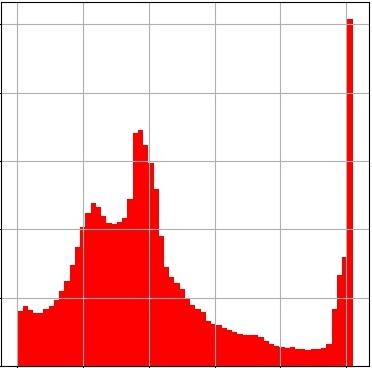
\includegraphics[scale=0.28]{tex/img/histgrered.jpg}
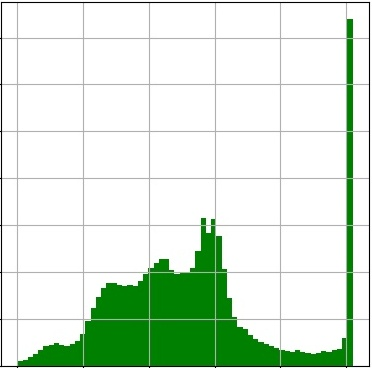
\includegraphics[scale=0.28]{tex/img/histgregreen.jpg}
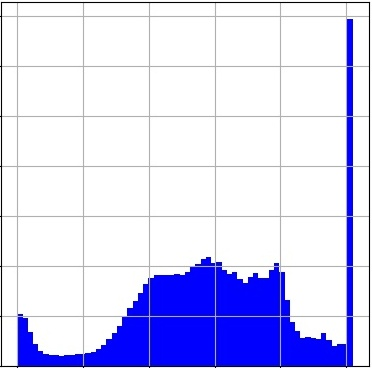
\includegraphics[scale=0.28]{tex/img/histgreblue.jpg}
	\caption{Distribution of byte value for each color of the original \textit{grenoble\_city.bmp} image}
\end{figure}

The X-axis of the histogram represents the byte value (between 0 and 255), and the Y-axis is the number of byte in the data for each value.

\begin{figure}[!h]
\centering
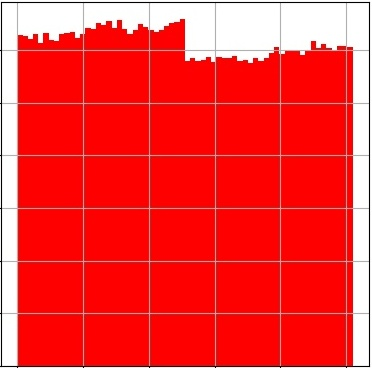
\includegraphics[scale=0.28]{tex/img/histgrered_en.jpg}
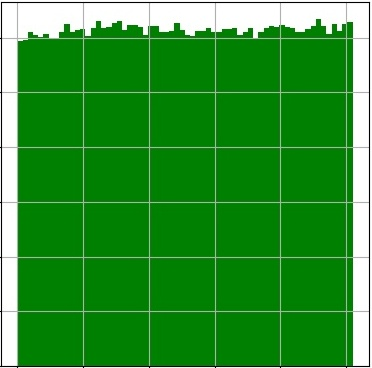
\includegraphics[scale=0.28]{tex/img/histgregreen_en.jpg}
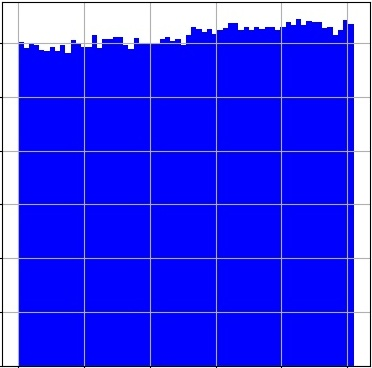
\includegraphics[scale=0.28]{tex/img/histgreblue_en.jpg}
	\caption{Distribution of byte value for each of the encrypted \textit{grenoble\_city.bmp} with a XOR key of two logistic maps ($\mu_1=3.89$, $r_{01}=0.6104$) and ($\mu_2=3.79$, $r_{02}=0.902$)} 
\end{figure}

In order to study the proposed algorithm, we're going to use the discrete chaotic map defined in the previous section.

We can observe on \textit{Figure 5} that the histograms of the encrypted images are completely different of the histograms of the original image. Furthermore, for each color, the distribution is almost uniform. We can conclude that the proposed algorithm is a good encryption algorithm in regards of the histogram analysis.
